% Hier befinden sich Textteil, die vielleicht noch gebraucht werden.s

%#########################################################################################

\begin{comment}
\begin{figure}[ht]
    \centering
    \begin{subfigure}[t]{0.52\textwidth}

      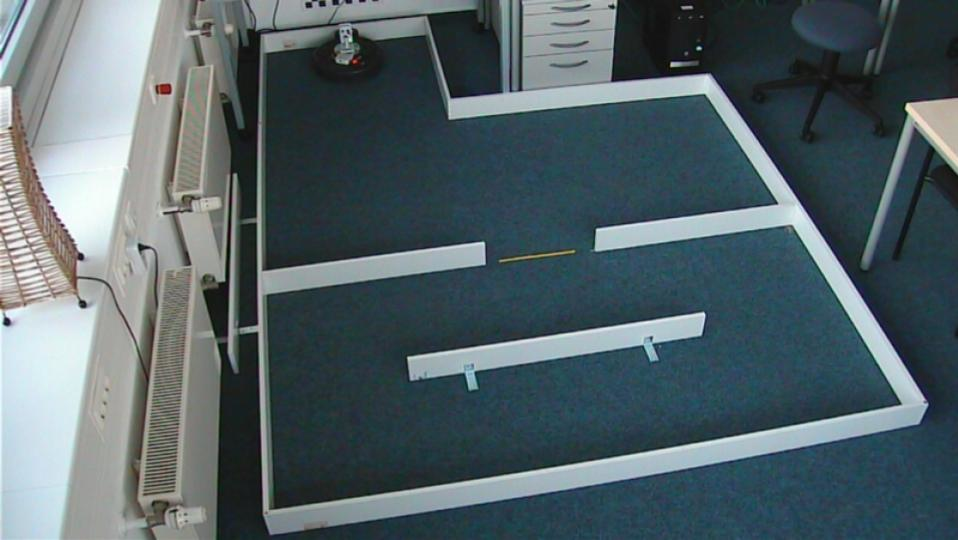
\includegraphics[scale=0.25]{bilder/evaluation/TopView.jpg}
        \caption{Sicht des aufgebauten Parcour}
        \label{fig:parcour}
     
    \end{subfigure}
    \vspace{0.2 cm}
    \begin{subfigure}[t]{0.45\textwidth}
      \includegraphics[scale=0.2]{bilder/evaluation/Parcour.png}
        \caption{zeigt das Auge von hinten mit dem austretendem Sehnerv}
        \label{fig:augeHinten}
    \end{subfigure}
    \caption{Die Muskulatur des rechten Augens}\label{fig:aufbauSchema}
\end{figure}
\end{comment}

%#################################################
\begin{figure}[h]
\begin{center}
\missingfigure{<Text> }
%\includegraphics[width=\textwidth, height=60mm]{bilder/grundlagen/auge_vorn.JPG}
\end{center}
\caption{\textbf{<Text>} <Text> }
\label{fig:<name>}
\end{figure}
%##################################################
\begin{figure}[ht]
    \centering
    \begin{subfigure}[t]{0.49\textwidth}
        \includegraphics[width=\textwidth, height=60mm]{bilder/grundlagen/auge_vorn.JPG}
        \caption{als Vorderansicht}
        \label{fig:augeVorne}
    \end{subfigure}
    \begin{subfigure}[t]{0.49\textwidth}
        \includegraphics[width=\textwidth, height=60mm]{bilder/grundlagen/auge_hinten.JPG}
        \caption{zeigt das Auge von hinten mit dem austretendem Sehnerv}
        \label{fig:augeHinten}
    \end{subfigure}
    \caption{Die Muskulatur des rechten Augens}\label{fig:rechtesAuge}
\end{figure}
%##############################################
\begin{figure}[ht]
   \begin{minipage}[b]{.25\linewidth} 
      \centering 
      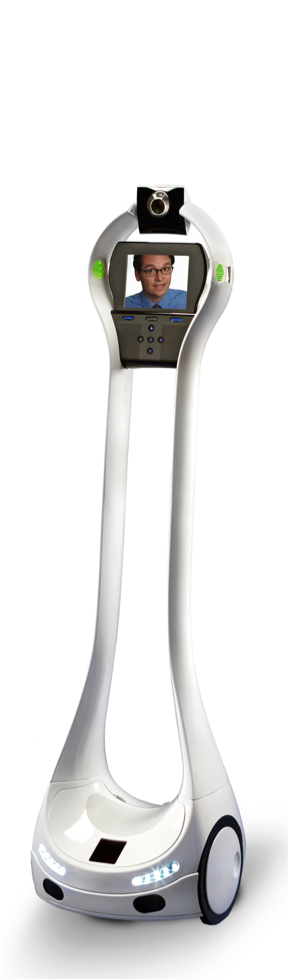
\includegraphics[width=0.7\textwidth]{bilder/grundlagen/1.png} 
      \subcaption{VGo}\label{fig:x} 
   \end{minipage}% 
   \hfill
   \begin{minipage}[b]{.25\linewidth} 
      \centering 
      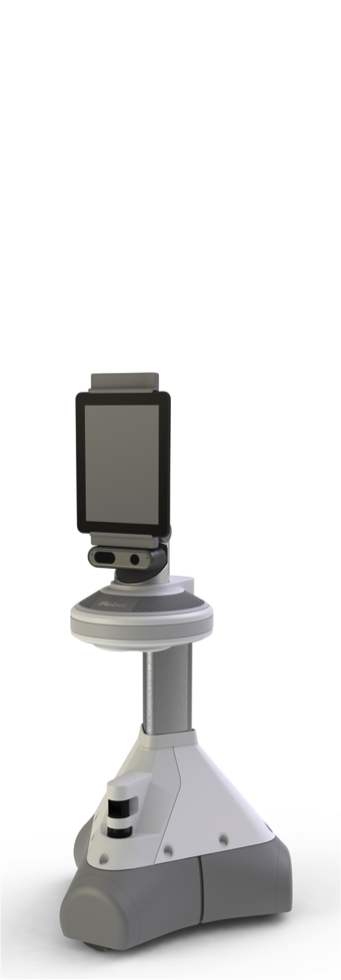
\includegraphics[width=0.9\textwidth]{bilder/grundlagen/2.png} 
      \subcaption{iRobot Ava}\label{fig:z} 
   \end{minipage}%
   \hfill
   \begin{minipage}[b]{.25\linewidth} 
      \centering 
      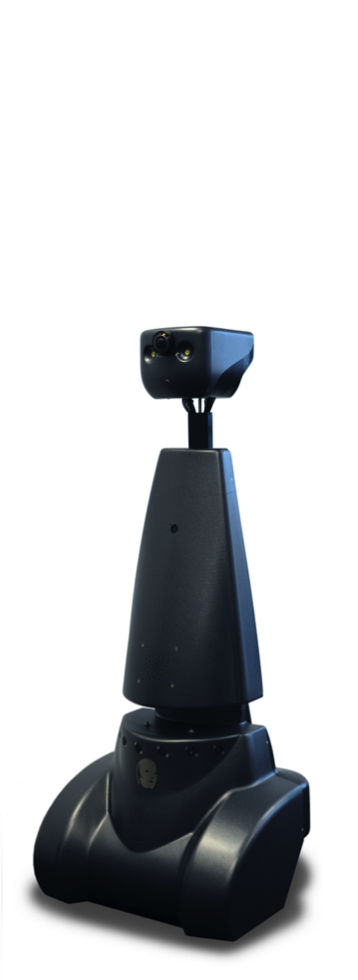
\includegraphics[width=0.9\textwidth]{bilder/grundlagen/3.png} 
      \subcaption{Gostai Jazz}\label{fig:y} 
   \end{minipage}%
   \hfill
   \begin{minipage}[b]{.25\linewidth} 
      \centering 
      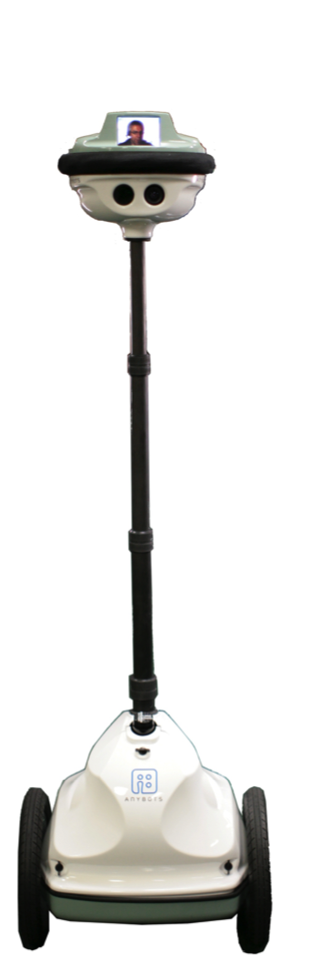
\includegraphics[width=0.7\textwidth]{bilder/grundlagen/4.png} 
      \subcaption{Anybots QB}\label{fig:z} 
   \end{minipage}%
   \hfill
   \caption{Alle Bilder}\label{fig:Bilder} 
\end{figure} 


%################################################
% Er enthält sechs Skalen mit insgesamt 18 Items in Form von Aussagen, die auf vierstufigen Ratingskalen hinsichtlich des Zutreffens der Aussage eingeschätzt werden. Dabei bedeuten: 1 = überhaupt nicht zutreffend, 2 = kaum zutreffend, 3 = ziemlich zutreffend, 4 = stark zutreffend und 5 = sehr stark zutreffend.
%################################################
\begin{comment}
% kapitel2.tex
\chapter{Grundlagen}
\label{chapter:grundlagen}

\section{Überblick}
\label{section:überblick}

Hier soll ein Überblick über Eytrackingsystme und der allgemeine Nutzen von Telepräsenzrobtersysteme stehen. Wie funktioniert allgemein die Steuerung von Robotern. 

\section{Der visuelle Informationstransfer vom Mensch zum Computer}
\label{section:informationstransfer}

\lipsum[4]

\section{Interpretation der Augeninformation durch den Eyetracker}
\label{section:XXX}

\section{Anwendungsgebiete von Eyetracking-Systemen}
\label{section:XXX}

\section{Anwendungsgebiete von \tp}
\label{section:XXX}

Die Anwendung von \tp wurde für verschiedene Anwendungsgebiete und Szenarien beschrieben. So beschreibt 


Grundsätzlich werden 2 Anwendungsscenarien für den Gebrauch von \tp benutzt. So beschreibt 
\end{comment}

%################################################
\begin{comment}

\begin{beispiel}{Befehlssequenz des \enquote{Drive}-Befehls in Rückwärtsrichtung in einer Geschwindigkeit von 200 mm/s: [137] [255] [56] [128] [0]} \\
%Befehls: [137] [0] [200] [128] [0]
%\textbf{[137] [255] [56] [1] [244]} \\
\(Opcode Drive Befehl= \textbf{[137]}\) \\
\(Geschwindigkeit = -200 = hex FF38 = [hex FF][hex 38] = \textbf{[255] [56]}\) \\
\(Radius= 0 = hex 8000 = [hex 80][hex 00] = \textbf{[128] [0]}\) \\
\label{exa:driveBack}
\end{beispiel}


\lstset{language=java, numbers=left, caption={Vorwärts}}
\begin{lstlisting}
int result = Math.abs(maxX - minX) + Math.abs(maxY - minY);  
if (result < maxDispersion && this.size() == maxBufferSize)
return Eyegesture.Fixation;
\end{lstlisting}

\begin{beispiel}{Befehlssequenz des \textsc{Drive}-Befehls in Vorwärtsrichtung in einer Geschwindigkeit von 200 mm/s: [137] [0] [200] [128] [0]} \\
%Befehls: [137] [0] [200] [128] [0]
%\textbf{[137] [255] [56] [1] [244]} \\
\(Opcode = \textbf{[137]}\) \\
\(Geschwindigkeit = 200 = hex 00C8 = [hex 00][hex C8] = \textbf{[0] [200]}\) \\
\(Radius= 0 = hex 8000 = [hex 80][hex 00] = \textbf{[128] [0]}\) \\
\label{exa:driveVor}
\end{beispiel}

\begin{beispiel}{Befehlssequenz des \enquote{Drive}-Befehls in Rückwärtsrichtung in einer Geschwindigkeit von 200 mm/s: [137] [255] [56] [128] [0]} \\
%Befehls: [137] [0] [200] [128] [0]
%\textbf{[137] [255] [56] [1] [244]} \\
\(Opcode = \textbf{[137]}\) \\
\(Geschwindigkeit = -200 = hex FF38 = [hex FF][hex 38] = \textbf{[255] [56]}\) \\
\(Radius= 0 = hex 8000 = [hex 80][hex 00] = \textbf{[128] [0]}\) \\
\label{exa:driveBack}
\end{beispiel}
\textcolor{red}{ Algorithmus folgt}


\end{comment}



%###################################################
\begin{comment}
% kapitel3.tex
\chapter{Fragestellung und Testmerkmale}
\label{chapter:fragestellung}

Zur Klärung der Arbeitsfragen: Machbarkeit, Präzision einer mobilen Robotersteuerung mithilfe eines Eyetrackers, sowie zur Klärung wie ermüdend diese Art der Steuerung ist und ob Unterschiede zwischen einer diskreten und kontinuierlichen Steuerungsform vorhanden sind wurde ein Fragebogen mit insgesamt 18 Fragen konzipiert. 
Ferner wurde die Quantifizierung der Zeit einer Parcourbewältigungsaufgabe als Merkmal festgelegt. Hierzu wurde ein Testparcour konzipiert, der einmalig mit jeder Steuerungsart umfahren werden muss. Die dabei benötigte Zeit ausgehend von einer festgelegten Start und Stoppposition werden aufgezeichnet und verglichen.


\section{Modellbildung}
\label{section:modellbildung}
Als Steuerungsmodi für den Roboter, soll eine \enquote{einfache} Basissteuerung sowie eine etwas anspruchsvollere Steuerung in Form einer Art \enquote{Joystick} realisiert werden.


\section{Steuerungsmodell}
\label{section:steurungsmodell}
Der vorgestellte Prototyp implementiert zwei unterschiedliche Steuerungsmodelle welche untereinander verglichen werden sollen. Es folgt eine Beschreibung dieser unterschiedlichen Steuermodelle mit den möglichen Bewegungsformen. 

\subsection{Diskretes Steuerungsmodell}
Das diskrete Steuerungsmodell stellt vier Unterschiedliche Bewegungen zur Verfügung. Hierbei werden zwei translationale Bewegungen in Vorwärts und in Rückwärtsrichtung angeboten, sowie jeweils die Rotation in- und entgegen des Uhrzeigersinnes. Somit ist diese Art der Steuerung vergleichbar mit einer \enquote{Art} Tastatursteuerung mit vier Tasten. Die Bewegung findet jeweils während der Betätigung der Tasten statt.

\subsection{Kontinuierliches Steuerungsmodell}
Das kontinuierliches Steuerungsmodell stellt eine anspruchsvollere Steuerung bereit. Hierbei wird mittels einer \enquote{Art} Joystick.

\section{Testmerkmale der Steuerung}
Als Merkmale die 


\end{comment}

%######################################
%The Roomba Open Interface (OI) is a software interface for controlling and manipulating Roomba’s behavior. The software interface lets you manipulate Roomba’s behavior and read its sensors through a series of commands, including mode commands, actuator commands, song commands, and sensor commands that you send to the Roomba’s serial port by way of a PC or microcontroller that is connected to the Mini-DIN connector.


%#####################################
\begin{beispiel}{Beispielsequenz eines \textsc{Drive}-Befehls: [137] [255] [56] [1] [244]} \\
\centering
\(
\underbrace{\color{orange}\underbrace{\underbrace{\text{\textsc{ Opcode }}}_{\substack{\text{\textsc{Drive}}}}}_{\substack{\text{\textsc{|137|}}}}
\color{blue}\underbrace{\underbrace{\underbrace{\text{\textsc{ Geschwindigkeit }}}_{\color{blue}\substack{\text{-200 mm/s}}}}_{\color{blue}\substack{hex FF38}}}_{\color{blue}\substack{\underbrace{hex FF}_{\substack{|255|}}\underbrace{hex 38}_{\substack{|56|}}}}\color{black}\underbrace{\underbrace{\underbrace{\text{\textsc{ Radius }}}_{\substack{\text{500 mm}}}}_{\substack{hex 01F4}}}_{\substack{\underbrace{hex 01}_{\substack{|1|}}\underbrace{hex F4}_{\substack{|244|}}}}} \)\\
\( [137] [255] [56] [1] [244] \)
%\( \underbrace{\underbrace{\text{\textsc{Opcode}}}_{\substack{\text{\textsc{Drive}}}}}_{\substack{\text{\textsc{|137|}}}} \underbrace{\underbrace{\underbrace{\text{\textsc{Geschwindigkeit}}}_{\substack{= \text{-200 mm/s}}}}_{\substack{\text{hex FF38}}}}\underbrace{\underbrace{\text{\textsc{Radius}}}_{\substack{= \text{500 mm}}}}_{\substack{\text{hex 01F4}}}\)
%\(\color{orange}\underbrace{\text{|137|}}_{\substack{\text{\textsc{Drive}}}}\color{blue}\underbrace{\underbrace{\underbrace{\text{|255|}}_{\substack{\text{hex FF}}} \underbrace{\text{|56|}}_{\substack{\text{hex 38}}}}_{\substack{= \text{-200 mm/s}}}}_{\substack{\text{\textsc{Geschwindigkeit}}}} \color{black}\underbrace{\underbrace{\underbrace{\text{|1|}}_{\substack{\text{hex 01}}}\underbrace{\text{|244|}}_{\substack{\text{hex F4}}}}_{\substack{= \text{500 mm}}}}_{\substack{\text{\textsc{Radius}}}}\) \\

\label{exa:drive}
\end{beispiel}


%#############################################

%\begin{beobachtung}{\textbf{\enquote{Drive Direct}-Befehl (Opcode: 145)} - allgemeine Struktur:} \\

%\noindent \textbf{[Opcode-Byte] [Geschwindigkeit rechtes Rad höherwertiges Byte] [Geschwindigkeit rechtes Rad niederwertiges Byte] [Geschwindigkeit linkes Rad höherwertiges Byte] [Geschwindigkeit rechtes linkes niederwertiges Byte]}.
%\end{beobachtung}

\begin{comment}
einen gewünschten Drehradius mittels des \enquote{Drive Direct}-Befehls zu realisieren. So lässt sich das Beispiel \ref{exa:drive} auf diese Weise mittels des \enquote{Drive Direct}-Befehl realisieren. \textcolor{red}{Geometrische umrechung mit darstellung falls die Zeit noch reicht.} %in nfach die Rotation um einen bestimmten Winkel zu ermöglichen. wie auch  Wie auch in der  Ist es beispielsweise vorgesehen den Roomba mit einer Geschwindigkeit von 200 mm/s in Rückwärtsrichtung (Geschwindigkeit mit negativem Vorzeichen) zu bewegen und Gleichzeit um einen Radius von 500 mm zu drehen, ergibt sich folgende Bytesequenz (Beispiel aus Manual): \\


\begin{beispiel}{Befehlssequenz des \enquote{Drive Direct}-Befehls: [145] [255] [56] [1] [244]} \\
%\textbf{[137] [255] [56] [1] [244]} \\ 
\(Opcode = \textbf{[137]}\) \\
\(Geschwindigkeit = -200 = hex FF38 = [hex FF][hex 38] = \textbf{[255] [56]}\) \\
\(Radius= 500 = hex 01F4 = [hex 01][hex F4] = \textbf{[1] [244]}\) \\
\label{exa:driveDirect}
\end{beispiel}
\end{comment}



\begin{comment}

\begin{table}[htp]
\begin{longtable}{|p{2cm}|p{2.5cm}|p{2cm}|p{2cm}|p{2cm}|p{2cm}|}
  \hline
Befehl & Befehls–opcode & Datenbyte 1 & Datenbyte 2 & Datenbyte 3 & Datenbyte 4 \\ 
  \hline
Start & 128 &  &  &  &  \\ 
Safe & 130 &  &  &  &  \\ 
Full & 131 &  &  &  &  \\ 
\hline
Drive & 137 & \multicolumn{2}{|p{4cm}|}{Geschwindigkeit (-500 – 500 mm/s)}   & Radius (-2000 – 2000 mm) &  \\ \hline
Drive Direct & 145 & Geschwindigkeit rechtes Rad (-500 – 500 mm/s) &  & Geschwindigkeit linkes Rad (-500 – 500 mm/s) &  \\ 
   \hline
\end{longtable}
\end{table}
Wie in der Tabelle zu erkennen ist besteht der \enquote{Start}-Befehls
\end{comment}


\begin{comment}
Für Personen mit Sprach- und Bewegungseinschränkungen sind jedoch die eigenen vier Wände häufig ohne Hilfe kaum zu erkunden. Der häufig einzige Kommunikationskanal wird durch eine Interaktion mit den Augen hergestellt. Die Entwicklung von Eyetracking-Systemen scheint in diesem Bereich neue Möglichkeiten zu bieten und den Betroffenen neue Interaktionswege zu eröffnen. Typischerweise findet die Kommunikation mittels Darstellungen von Schriftzeichen auf einem Bildschirm statt, wobei durch den Benutzer durch sequentiell auswahl einzelner Zeichen Wörter gebildet werden und diese schließlich zu Sätzen aneinander gereiht werden. Welche Möglichkeiten durch diese Augmentation der Kommunikation gegeben werden zeigt nicht nur das prominete Beispiel von Steve Hawking.

In Deutschland leiden 

Die vorliegende Arbeit baut auf den gewonnen Erkenntnissen von Eidam et al. auf und erweitert diese um eine virtuelles Präsenz System (VPS). Hierdurch wird eine aktuelle \enquote{live} Ansicht der Umgebung ermöglicht. Ferner wird dem Benutzer eine Möglichkeit zur Steuerung des VPS gegeben. Dadurch erweitern sich die Möglichkeiten der Interaktion um ein vielfaches. Es soll eine Interaktion mit Alltagsgegenständen ermöglicht werden (z.B. Betätigen des Lichtschalters) 

die durch den Benutzer mittels Augengeste mühsam Die Erhaltung der Autonomie und der Kommunikation scheinen kann ein Leben so normal wie möglich ermöglichen. 

Diese Abhängigkeit manifestiert sich in ganz alltäglichen Lebensbereichen und führt zu einer Verbesserung der nötigsten Fähigkeiten. 

Die Fähigkeit der differenzierten Kommunikation ist eine der Grundlegenden Menschlichen Fähigkeiten. Ohne diese Möglichkeiten wäre eine Teilnahme an täglichen Lebensbereichen kaum möglich. Patientin mit Einschränkungen im Bereich der Locked-in Syndrome (LIS) haben nur eine begrenzte Möglichkeit mit ihrer Umwelt zu kommunizieren um ihre Wünsche zu artikulieren. 

Amyothropher Lateralsklerose (ALS) ist eine neurodegenerative Erkrankung welche zu einer progressiven Paralyse der willkürlichen Muskulatur führt. Die Erkrankten verlieren ihre Fähigkeit sich zu Bewegen oder zu sprechen, aber bis zuletzt nicht die Fähigkeit der Augenbewegung.

Im Rahmen dieser Abschlussarbeit soll ein Softwareprototyp realisiert werden, der es ermöglicht mit Hilfe definierter Augengesten einen beweglichen Roboter (iRobot Roomba 620) zu steuern. Die Augengestenerkennung erfolgt mittels eines stationären Eyetrackingsystems (Systems RED von SensoMotoric Instruments GmbH), welches an einem Bildschirm angebracht ist. Hierbei ermöglicht eine am Roboter angebrachte Kamera eine \enquote{Live-Ansicht} der Umgebung aus \enquote{Sicht} des Roboters und präsentiert dies auf den Stimuluspräsentierenden Bildschirm, welcher vom Eyetracker \enquote{überwacht} wird. Primär soll in der Arbeit die Frage der Machbarkeit und die Frage der Präzision einer derartigen Mensch-Roboter-Interaktion geklärt werden. Ferner soll abgeschätzt werden, wie ermüdend diese Art der Steuerung ist und ob Unterschiede zwischen den verschiedenen Steuerungssystemen vorhanden sind. Außerdem soll eine Art \enquote{Panikschalter}, also ein sofortiger Stopp des Roboters umgesetzt werden.
 
Das Störungsbild Locked-in Syndrom (LiS) kann als Folge verschiedener Schädigungen des Gehirns auftreten, häufigste Ursache sind zerebrovaskuläre Erkrankungen wie Hirninfarkte oder intrazerebrale Blutungen. 

\end{comment}


%%%%%%%%%%%%%%%%%%%%%%%%%%%#################################################
%%%%%%%%%%%%%%%%%%%%%%%%%%%#################################################
%%%%%%%%%%%%%%%%%%%%%%%%%%%#################################################

% kapitel4.tex
\chapter{Implementierung}
\label{chapter:implementierung}
Das folgende Kapitel stellt die in Abschnitt \ref{section:steurungsmodell} beschriebenen Modelle und deren Implementierung im entwickelten Softwareprototypen dar. Ferner wird auf die technischen Komponenten, das Eyetracking-System RED der Firma SensoMotoric Instruments GmbH (SMI) und das mobilen Robotersystems (Roomba 620) der Firma iRobot® Corporation, konkret eingegangen.

\section{Telepräsenzrobotersytem}
\subsection{iRobot Roomba 620}
Für die vorliegende Arbeit wurde als \tp ein \enquote{handelsüblicher} autonomer Staubsaugerroboter (Roomba 620) der Firma iRobot® Corporation verwendet, siehe Abbildung \ref{fig:roomba}. Der Roomba ist seitens des Herstellers so konzipiert worden, dass dieser ohne technische Vorkenntnisse des Benutzers relativ einfach verwendet werden kann und hierbei weitgehend autonom funktioniert. Jedoch eignet sich der Roomba aufgrund einer seit 2005 vom Hersteller bereitgestellten offene Schnittstellendokumentation (iRoomba Create Open Interface (ROI)) (Lit einfügen!!!), hervorragend zur Augmentation als \tp. Der Roomba ist somit im Verhalten durch die bereitgestellte Befehelsstruktur der ROI vielfältig zu kontrollieren. Um die für ein \tp benötigte \enquote{Live}-Ansicht zu ermöglichen wurde der Roboter um eine zentrisch angeordnete Kamera der Firma Axis (AXIS M1034-W) erweitert, siehe Abbildung (modifizierter Roomba). Die vorinstallierten Bürsten des Staubsaugerroboters wurden aufgrund der Geräuschentwicklung entfernt. Zur Netzwerkkommunikation und entfernten Steuerung wurde ein Access-Point am mobilen Roboter angebracht. Dieser dient als Verbindung zum seriellen Anschluss des Roboters und wird über \enquote{socat}-Prozesse gesteuert. 


\begin{figure}[ht]
\begin{center}
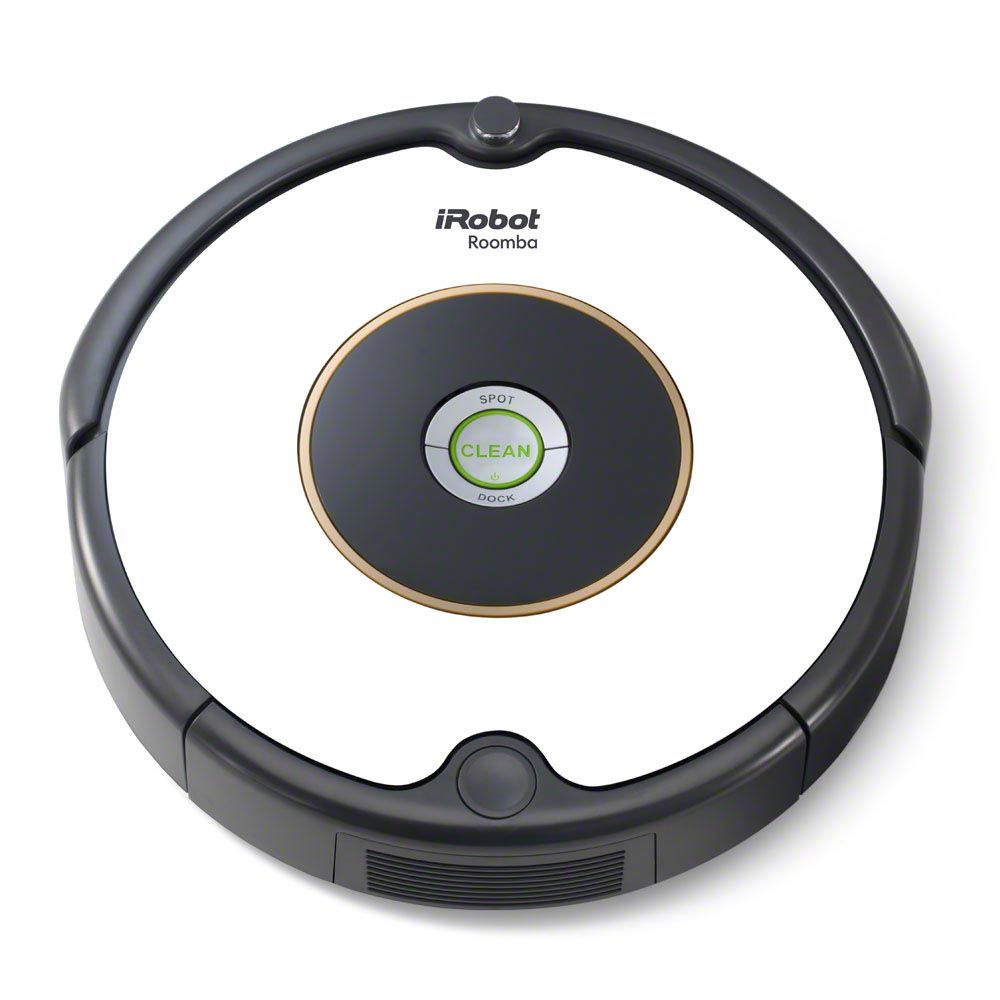
\includegraphics[scale=0.1]{bilder/implementierung/Roomba.jpg}
\end{center}
\caption{Roomba 620}
\label{fig:roomba}
\end{figure}
\footnote{\url{http://shop.irobot.de/roomba-staubsstaubsaugerroboter-roomba-605/R605040.html?cgid=de&lang=de_DE} zuletzt besucht am 23. November 2016}

Nachfolgend erfolgt die Vorstellung der Schnittstellendokumentation mit der Einführung in die bereitgestellten Kontrollmodi und die für die Implementierung benötigten Befehle.

\subsection{Modi des iRoomba Create Open Interface (ROI)}
Bei der Benutzung des ROI befindet sich der Roomba in einem der vier unterschiedlichen Kontrollmodi: Off, Passiv, Safe und Full (iRobot Manual). Die Modi legen fest, welche Verhaltensweisen seitens des Roombas vorgesehen sind und wie auf eintreffende Befehle \ref{subsction:befehlsstruktur}) reagiert wird. Folgend werden die vier Modi des Roombas wie in den Angaben des Herstellers beschrieben
dargestellt \footnote{\url{https://www.irobot.com/filelibrary/pdfs/hrd/create/Create\%20Open\%20Interface_v2.pdf}}:

\textbf{\enquote{Off}-Modus}: Nach einem Batteriewechsel oder nach dem ersten Anschalten des Roombas befindet sich der Roomba in diesem Modus. Der Roomba erwartet in diesem Modus ein \enquote{Start}-Befehl (siehe \ref{subsction:befehlsstruktur}) und wechselt nach erhalten des Befehls in den \enquote{Passiv}-Modus.

\textbf{\enquote{Passiv}-Modus}: Nach erhalten eines \enquote{Start}-Befehls (siehe \ref{subsction:befehlsstruktur}) wechselt der Roomba in diesen Modus. Hierbei können Sensordaten ausgelesen werden, jedoch sind keine Steuerbefehle für die vorhandenen Steuerkomponenten (Lautsprecher, Motoren, Leuchtdioden) möglich. 

\textbf{\enquote{Safe}-Modus}: Der Safe-Modus bietet die gleiche Funktionalität wie der Passiv-Modus. Zusätzlich kann der Roomba hierbei nun kontrolliert und gezielt gesteuert werden. Alle vorhandenen Befehle sind nun ausführbar unter der Voraussetzung, dass keiner der folgenden Sicherheitsrelevanten Ereignisse eingetreten ist: 
\begin{itemize}
\item Ein Abhang wird während der Vorwärts- oder Rückwärtsbewegung erkannt.
\item Ein Rad steckt fest.
\item Das Ladegerät ist angeschlossen und der Roomba wird geladen.
\end{itemize}
Tritt einer dieser Sicherheitsrelevanten Ereignisse auf werden alle Motoren umgehend gestoppt und der Roomba wird in den \enquote{Passiv}-Mode versetzt.

\textbf{\enquote{Full}-Modus}: Durch das Senden eines \enquote{Full}-Befehls (siehe \ref{subsction:befehlsstruktur}) erhält der Benutzer im vollen Umfang Zugang zu den Steuerkomponenten (Lautsprecher, Motoren, Leuchtdioden). Die Sicherheitsrelevanten Ereignisse werden hierbei nicht überwacht.

\textcolor{red}{hier noch einen Satz im Bezug auf den Prototypen  verwendeten Modi. Zur Verdeutlichung kann noch eine eigene Darstellung der Modi hinzugefügt werden. }

%The Roomba Open Interface (OI) is a software interface for controlling and manipulating Roomba’s behavior. The software interface lets you manipulate Roomba’s behavior and read its sensors through a series of commands, including mode commands, actuator commands, song commands, and sensor commands that you send to the Roomba’s serial port by way of a PC or microcontroller that is connected to the Mini-DIN connector.

\subsection{Befehlsstruktur des iRoomba Create Open Interface (ROI)}
\label{subsction:befehlsstruktur}
Der Befehlsumfang welche durch das ROI angeboten wird, bietet eine umfangreiche Interaktionsmöglichkeit mit den Sensoren und Steuerkomponenten des Roombas. Für die Implementierung des Softwareprototyps war nur eine kleine Anzahl der bereitgestellten Befehle notwendig. Die nachfolgende Auflistung führt somit nur die für die Implementierung verwendeten Befehle auf. Für eine vollständige Auflistung der angebotenen Befehle sei auf die ausführlichen Angaben des Herstellers verwiesen (Lit Rommba manual). 

\begin{itemize}
\item \textbf{\enquote{\textsc{Start}}} (Opcode: 128) (Datenbytes: 0)
\item \textbf{\enquote{SAFE}} (Opcode: 131) (Datenbytes: 0)
\item \textbf{\enquote{FULL}} (Opcode: 132) (Datenbytes: 0)
\item \textbf{\enquote{POWER}} (Opcode: XXX) (Datenbytes: 0)
\item \textbf{\enquote{DOCK}} (Opcode: XXX) (Datenbytes: 0)
\item \textbf{\enquote{DRIVE}} (Opcode: 137) (Datenbytes: 4)
\item \textbf{\enquote{DRIVE DIRECT}} (Opcode: 145) (Datenbytes: 4)
\end{itemize}

Jeder ROI-Befehl beginnen mit einem Ein-Byte großen Befehlsopcode der den gewünschten Befehl kodiert. In Abhängigkeit des Befehlsopcodes werden zusätzlich einer oder mehrere weitere Datenbytes als Argument des Befehls benötigt.
\begin{equation*}
\noindent \color{black} \underbrace{\textbf{|OPCODE|}}_{\substack{\text{Befehlsauswahl}}}\hfill \color{black}\underbrace{\textbf{|Datenbyte 1|}\hfill \textbf{|Datenbyte 2|} \hfill \textbf{|Datenbyte 3|}\hfill \textbf{|Datenbyte 4|}}_{\substack{\text{Variable Anzahl der Datenbytes in Abhänigkeit des Befehlsopcods}}} \hfill 
\end{equation*}

Viele Befehle wie beispielsweise der oben bereits genannte \textbf{\enquote{Start}-Befehl (Opcode: 128)} benötigen keine zusätzlichen Datenbytes. Auch die Gruppe der Modus-Befehle wie beispielsweise der \textbf{\enquote{Safe}-Befehl (Opcode: 131)}, der den Roomba in den \enquote{Safe}-Modus versetzt, oder der \textbf{\enquote{Full}-Befehl (Opcode: 132)}, womit der Roomba in den \enquote{Full}-Modus wechselt, benötigen keine weiteren Datenbytes. 

Für die Umsetzung der diskreten und kontinuierlichen Steuerung wurden zwei unterschiedliche Steuerungsbefehle verwendet. Für die diskrete Steuerung bot sich die Funktionsweise des \textbf{\enquote{Drive}-Befehls (Opcode: 137)} an. Bei der kontinuierlichen Steuerung wurde die Funktion des \textbf{\enquote{Drive Direct}-Befehl (Opcode: 145)} verwendet. Es folgt nun eine allgemeine Beschreibung dieser beiden Befehle. Die konkrete Anwendung folgt in den Abschnitten \ref{subsection:diskSt} \bzw \ref{subsection:kontSt}.


\subsubsection{\textsc{Drive}-Befehl (Opcode: 137)}
Für die Steuerung mittels \textsc{Drive}-Befehl (Opcode: 137) wurde die Ansteuerung der beiden Radmotoren des Roombas durch die Angabe zweier Argumente realisiert (Geschwindigkeit, Radius).
Hierbei erfolgte die Steuerung durch die Angabe einer durch zwei Bytes kodierten \textbf{Geschwindigkeit} im Bereich von -500 mm/s bis \mathplus 500 mm/s kombiniert mit der Angabe eines durch weitere zwei Bytes kodierten \textbf{Radius} im Bereich von -2000 mm bis \mathplus 2000 mm. Daraus ergibt sich für den \textsc{Drive}-Befehl die allgemeine \textbf{sequenzielle Struktur} des Befehls:
\begin{equation*}
\begin{split}
\underbrace{\underbrace{\text{|137|}}_{\substack{\text{\text{1 Byte}}}}}_{\substack{\text{\textsc{opcode}}}} \underbrace{\underbrace{\text{|höherwertiges Byte|}}_{\substack{\text{1 Byte}}} \underbrace{\text{|niederwertiges Byte|}}_{\substack{\text{1 Byte}}}}_{\substack{\text{\textsc{Geschwindigkeit}}}} \underbrace{\underbrace{\text{|höherwertiges Byte|}}_{\substack{\text{1 Byte}}} \underbrace{\text{|niederwertiges Byte|}}_{\substack{\text{1 Byte}}}}_{\substack{\text{\textsc{Radius}}}}
\end{split}
\end{equation*}

Anhand der allgemeinen Struktur des \textsc{Drive}-Befehls kann man erkennen, dass zusätzlich zum Opcode-Byte vier weiter Datenbytes notwendig sind, die als zwei vorzeichenbehaftete 16-Bit Zahlen in Zweierkomplementdarstellung vorliegen. Hierbei erkennt man ferner, dass eine Big-Endian Byte-Reihenfolge vorgesehen ist und das höchstwertige Byte zuerst angegeben werden muss. Ist es beispielsweise vorgesehen den Roomba mit einer Geschwindigkeit von 200 mm/s in Rückwärtsrichtung (Geschwindigkeit mit negativem Vorzeichen) zu bewegen und Gleichzeit in einen Radius von 500 mm zu drehen, ergibt sich folgende Bytesequenz des Befehls (Beispiel aus Manual):
\begin{beispiel}{Beispielsequenz eines \textsc{Drive}-Befehls: [137] [255] [56] [1] [244]} \\
\centering
\(
\underbrace{\color{orange}\underbrace{\underbrace{\text{\textsc{ Opcode }}}_{\substack{\text{\textsc{Drive}}}}}_{\substack{\text{\textsc{|137|}}}}
\color{blue}\underbrace{\underbrace{\underbrace{\text{\textsc{ Geschwindigkeit }}}_{\color{blue}\substack{\text{-200 mm/s}}}}_{\color{blue}\substack{hex FF38}}}_{\color{blue}\substack{\underbrace{hex FF}_{\substack{|255|}}\underbrace{hex 38}_{\substack{|56|}}}}\color{black}\underbrace{\underbrace{\underbrace{\text{\textsc{ Radius }}}_{\substack{\text{500 mm}}}}_{\substack{hex 01F4}}}_{\substack{\underbrace{hex 01}_{\substack{|1|}}\underbrace{hex F4}_{\substack{|244|}}}}} \)\\
\( [137] [255] [56] [1] [244] \)
%\( \underbrace{\underbrace{\text{\textsc{Opcode}}}_{\substack{\text{\textsc{Drive}}}}}_{\substack{\text{\textsc{|137|}}}} \underbrace{\underbrace{\underbrace{\text{\textsc{Geschwindigkeit}}}_{\substack{= \text{-200 mm/s}}}}_{\substack{\text{hex FF38}}}}\underbrace{\underbrace{\text{\textsc{Radius}}}_{\substack{= \text{500 mm}}}}_{\substack{\text{hex 01F4}}}\)
%\(\color{orange}\underbrace{\text{|137|}}_{\substack{\text{\textsc{Drive}}}}\color{blue}\underbrace{\underbrace{\underbrace{\text{|255|}}_{\substack{\text{hex FF}}} \underbrace{\text{|56|}}_{\substack{\text{hex 38}}}}_{\substack{= \text{-200 mm/s}}}}_{\substack{\text{\textsc{Geschwindigkeit}}}} \color{black}\underbrace{\underbrace{\underbrace{\text{|1|}}_{\substack{\text{hex 01}}}\underbrace{\text{|244|}}_{\substack{\text{hex F4}}}}_{\substack{= \text{500 mm}}}}_{\substack{\text{\textsc{Radius}}}}\) \\

\label{exa:drive}
\end{beispiel}

Der \textsc{Drive}-Befehl stellt für einige Bewegungsrichtungen wie die Rotation in- oder entgegen des Uhrzeigersinn, sowie die Geradausfahrt in Vorwärts und Rückwärtsrichtung spezielle Werte des Radius-Parameters bereit (Lit Manual):

\begin{itemize}
  \item Gerade = 32768 oder 32767 = hex 8000 oder 7FFF
  \item Rotation in Uhrzeigersinn = hex FFFF
  \item Rotation entgegen des Uhrzeigersinn = hex 0001
\end{itemize}

Der \textsc{Drive}-Befehl kann, wie oben erwähnt, nur während der Ausführung im \enquote{Safe}-oder \enquote{Full}-Modus verwendet werden. Das oben genannte Beispiele zeigt die allgemeine Befehlsstruktur des von der ROI bereitgestellten \textsc{Drive}-Befehls (Opcode: 137). 


\subsubsection{\textsc{Drive} \textsc{Direct}-Befehl (Opcode: 145)}
Der \textsc{Drive} \textsc{Direct}-Befehl (Opcode: 145) unterscheidet sich zum o.g. \textsc{Drive}-Befehl dahingehend, dass die Ansteuerung der einzelnen Radsteuermotoren für jedes Rad einzeln möglich ist. Auf diese Art und Weise lässt sich die für die kontinuierliche Steuerung notwendige differenzierte kontinuierliche geschwindigkeits- und richtungsabhängige Befehlscodierung in einem einfachen Algorithmus implementieren, siehe Abschnitt \ref{subsection:kontSt}. Es folgt die allgemeine sequenzielle Struktur des \textsc{Drive} \textsc{Direct}-Befehls (Opcode: 145):
\begin{equation*}
\begin{split}
\underbrace{\underbrace{\text{|145|}}_{\substack{\text{\text{1 Byte}}}}}_{\substack{\text{\textsc{opcode}}}} \underbrace{\underbrace{\text{|höherwertiges Byte|}}_{\substack{\text{1 Byte}}} \underbrace{\text{|niederwertiges Byte|}}_{\substack{\text{1 Byte}}}}_{\substack{\text{\textsc{Geschwindigkeit rechtes Rad}}}} \underbrace{\underbrace{\text{|höherwertiges Byte|}}_{\substack{\text{1 Byte}}} \underbrace{\text{|niederwertiges Byte|}}_{\substack{\text{1 Byte}}}}_{\substack{\text{\textsc{Geschwindigkeit linkes Rad}}}}
\end{split}
\end{equation*}

Anhand der allgemeinen Struktur des \textsc{Drive} \textsc{Direct}-Befehls erkennt man, dass genau wie beim \textsc{Drive}-Befehl zusätzlich zum Opcode-Byte vier weiter Datenbytes benötigt werde. Auch hierbei handelt es sich um zwei 16-Bit Zahlen in Zweierkomplementärdarstellung und in Big-Endian Byte-Reihenfolge.
Ein konkretes Beispiel verdeutlicht die Nutzung des \textsc{Drive} \textsc{Direct}-Befehls:

\begin{beispiel}{Beispielsequenz eines \textsc{Drive} \textsc{Direct}-Befehls: [145] [0] [200] [0] [200]} \\
%\textbf{[137] [255] [56] [1] [244]} \\ 
\centering
\(\color{orange}\underbrace{\text{|145|}}_{\substack{\text{\textsc{Drive}\textsc{Direct }}}}\color{blue}\underbrace{\underbrace{\underbrace{\text{|0|}}_{\substack{\text{hex 00}}} \underbrace{\text{|200|}}_{\substack{\text{hex C8}}}}_{\substack{= \text{200 mm/s}}}}_{\substack{\text{\textsc{Geschwindigkeit rechtes Rad }}}} \color{black}\underbrace{\underbrace{\underbrace{\text{|0|}}_{\substack{\text{hex 00}}} \underbrace{\text{|200|}}_{\substack{\text{hex C8}}}}_{\substack{= \text{200 mm/s}}}}_{\substack{\text{\textsc{Geschwindigkeit linkes Rad }}}}\)
\label{exa:driveDirect}
\end{beispiel}

Die erzeugte Bewegung der Befehlssequenz im Beispiel \ref{exa:driveDirect} entspräche einer Fahrt mit einer Geschwindigkeit von 200 mm/s gerade aus, da beide Motoren die gleiche Geschwindigkeit umsetzen.

Die Umsetzung des \textsc{Drive} \textsc{Direct}-Befehls kann ebenfalls nur während der Ausführung im \enquote{Safe}- oder \enquote{Full}-Modus erfolgen. 

Nachfolgend wird auf die konkrete Umsetzung, der beschriebenen Befehle (\textsc{Drive}-Befehls (Opcode: 137), \textsc{Drive} \textsc{Direct}-Befehl (Opcode: 145)) für die Steuermodelle eingegangen und die Anwendung der Befehle nochmals verdeutlicht.

%\begin{beobachtung}{\textbf{\enquote{Drive Direct}-Befehl (Opcode: 145)} - allgemeine Struktur:} \\

%\noindent \textbf{[Opcode-Byte] [Geschwindigkeit rechtes Rad höherwertiges Byte] [Geschwindigkeit rechtes Rad niederwertiges Byte] [Geschwindigkeit linkes Rad höherwertiges Byte] [Geschwindigkeit rechtes linkes niederwertiges Byte]}.
%\end{beobachtung}

\begin{comment}
einen gewünschten Drehradius mittels des \enquote{Drive Direct}-Befehls zu realisieren. So lässt sich das Beispiel \ref{exa:drive} auf diese Weise mittels des \enquote{Drive Direct}-Befehl realisieren. \textcolor{red}{Geometrische umrechung mit darstellung falls die Zeit noch reicht.} %in nfach die Rotation um einen bestimmten Winkel zu ermöglichen. wie auch  Wie auch in der  Ist es beispielsweise vorgesehen den Roomba mit einer Geschwindigkeit von 200 mm/s in Rückwärtsrichtung (Geschwindigkeit mit negativem Vorzeichen) zu bewegen und Gleichzeit um einen Radius von 500 mm zu drehen, ergibt sich folgende Bytesequenz (Beispiel aus Manual): \\


\begin{beispiel}{Befehlssequenz des \enquote{Drive Direct}-Befehls: [145] [255] [56] [1] [244]} \\
%\textbf{[137] [255] [56] [1] [244]} \\ 
\(Opcode = \textbf{[137]}\) \\
\(Geschwindigkeit = -200 = hex FF38 = [hex FF][hex 38] = \textbf{[255] [56]}\) \\
\(Radius= 500 = hex 01F4 = [hex 01][hex F4] = \textbf{[1] [244]}\) \\
\label{exa:driveDirect}
\end{beispiel}
\end{comment}



\begin{comment}

\begin{table}[htp]
\begin{longtable}{|p{2cm}|p{2.5cm}|p{2cm}|p{2cm}|p{2cm}|p{2cm}|}
  \hline
Befehl & Befehls–opcode & Datenbyte 1 & Datenbyte 2 & Datenbyte 3 & Datenbyte 4 \\ 
  \hline
Start & 128 &  &  &  &  \\ 
Safe & 130 &  &  &  &  \\ 
Full & 131 &  &  &  &  \\ 
\hline
Drive & 137 & \multicolumn{2}{|p{4cm}|}{Geschwindigkeit (-500 – 500 mm/s)}   & Radius (-2000 – 2000 mm) &  \\ \hline
Drive Direct & 145 & Geschwindigkeit rechtes Rad (-500 – 500 mm/s) &  & Geschwindigkeit linkes Rad (-500 – 500 mm/s) &  \\ 
   \hline
\end{longtable}
\end{table}
Wie in der Tabelle zu erkennen ist besteht der \enquote{Start}-Befehls
\end{comment}

 
\section{Umsetzung der Robotersteuerung}

Nachdem die Befehlsstruktur der Schnittstelle des Roombas im vorherigen Kapitel beschrieben wurde folgt nun die konkrete Anwendung der Befehle im Rahmen der beiden Steuerungsmethoden. 

\subsection{Umsetzung der diskreten Steuermethode}
\label{subsection:diskSt}
Unter dem Begriff des diskrete Steuermodells, wie es in der vorliegenden Arbeit verwendet wird, ist eine Steuermethode zu verstehen, die nur während gezielter Betätigung eines Steuerelementes ein vorgegebenes positives Bewegungssignal erzeugt. Fehlt diese Betätigung findet kein Signalerzeugung statt. Dies unterscheidet sich beim kontinuierlichen Steuerungsmodell. Hierbei wird  kontinuierlich ein Signal verarbeitet findet eine quasi kontinuierliche Steuerung statt
Zur Umsetzung der diskreten Steuerungen wurden vier Steuerelemente (Vor, Zurück, Links, Rechts) auf dem Bildschirm angeordnet, siehe Abbildung \ref{fig:diskretMode}. Findet nun eine Blickgeste (siehe Kapitel \ref{section:augengestenerkennung}) in einen Bereich eines der Steuerelemente statt, so wird der entsprechende Befehl an den mobilen Roboter gesendet. Hierbei wird beispielsweise durch das \enquote{Vor} Steuerelement das Signal einer translationalen Bewegung in Vorwärtsrichtung in der aktuellen Geschwindigkeit an den mobilen Roboter gesendet. Durch das Steuerelement \enquote{Zurück} entsprechend in Rückwärtsrichtung. Verlässt der POR des Benutzers den Bereich des Steuerelementes wird dementsprechend kein weiteres Signal gesendet. Wird durch eine Blickgeste eines der \enquote{Links} oder \enquote{Rechts}-Steuerelemente ausgewählt, so wird ein Befehl zur Rotation in- oder entgegen des Uhrzeigersinn an der aktuellen Position an den mobilen Roboter gesendet. Eine translationale Bewegung findet hierbei nicht statt. Auch hierbei wird beim Verlassen der Blickbewegung des jeweiligen Steuerelementes, die entsprechende Rotationsbewegungsbewegung gestoppt. Durch diese Art der Steuerung sind durch alternierende Rotation und Translationsbewegungen jegliche Positionen auf dem Feld zu erreichen und die geplante Parcourbewältigungsaufgabe zu bewältigen. Wie bereits im Kapitel \ref{subsction:befehlsstruktur} dargelegt, wurde zur Umsetzung der Steuerkomponenten der diskreten Steuerung der Befehl \textsc{Drive} verwendet. Hierbei wurde jeder Steuerkomponente (Vor, Zurück, Links, Rechts) die beabsichtigte Bewegungsrichtung durch die feste Zuteilung der Befehlsparameter (Geschwindigkeit, Radius) für eine der vier möglichen Bewegungen zugewiesen. Die programmiertechnische Umsetzung erfolgte mittels Command-Muster, \vgl (Kapitel architektur). 

\lstset{language=java, numbers=left, caption={Vorwärts}}
\begin{lstlisting}
int result = Math.abs(maxX - minX) + Math.abs(maxY - minY);  
if (result < maxDispersion && this.size() == maxBufferSize)
return Eyegesture.Fixation;
\end{lstlisting}

\begin{beispiel}{Befehlssequenz des \textsc{Drive}-Befehls in Vorwärtsrichtung in einer Geschwindigkeit von 200 mm/s: [137] [0] [200] [128] [0]} \\
%Befehls: [137] [0] [200] [128] [0]
%\textbf{[137] [255] [56] [1] [244]} \\
\(Opcode = \textbf{[137]}\) \\
\(Geschwindigkeit = 200 = hex 00C8 = [hex 00][hex C8] = \textbf{[0] [200]}\) \\
\(Radius= 0 = hex 8000 = [hex 80][hex 00] = \textbf{[128] [0]}\) \\
\label{exa:driveVor}
\end{beispiel}

\begin{beispiel}{Befehlssequenz des \enquote{Drive}-Befehls in Rückwärtsrichtung in einer Geschwindigkeit von 200 mm/s: [137] [255] [56] [128] [0]} \\
%Befehls: [137] [0] [200] [128] [0]
%\textbf{[137] [255] [56] [1] [244]} \\
\(Opcode = \textbf{[137]}\) \\
\(Geschwindigkeit = -200 = hex FF38 = [hex FF][hex 38] = \textbf{[255] [56]}\) \\
\(Radius= 0 = hex 8000 = [hex 80][hex 00] = \textbf{[128] [0]}\) \\
\label{exa:driveBack}
\end{beispiel}
\textcolor{red}{ Algorithmus folgt}

\begin{figure}[ht]
\begin{center}
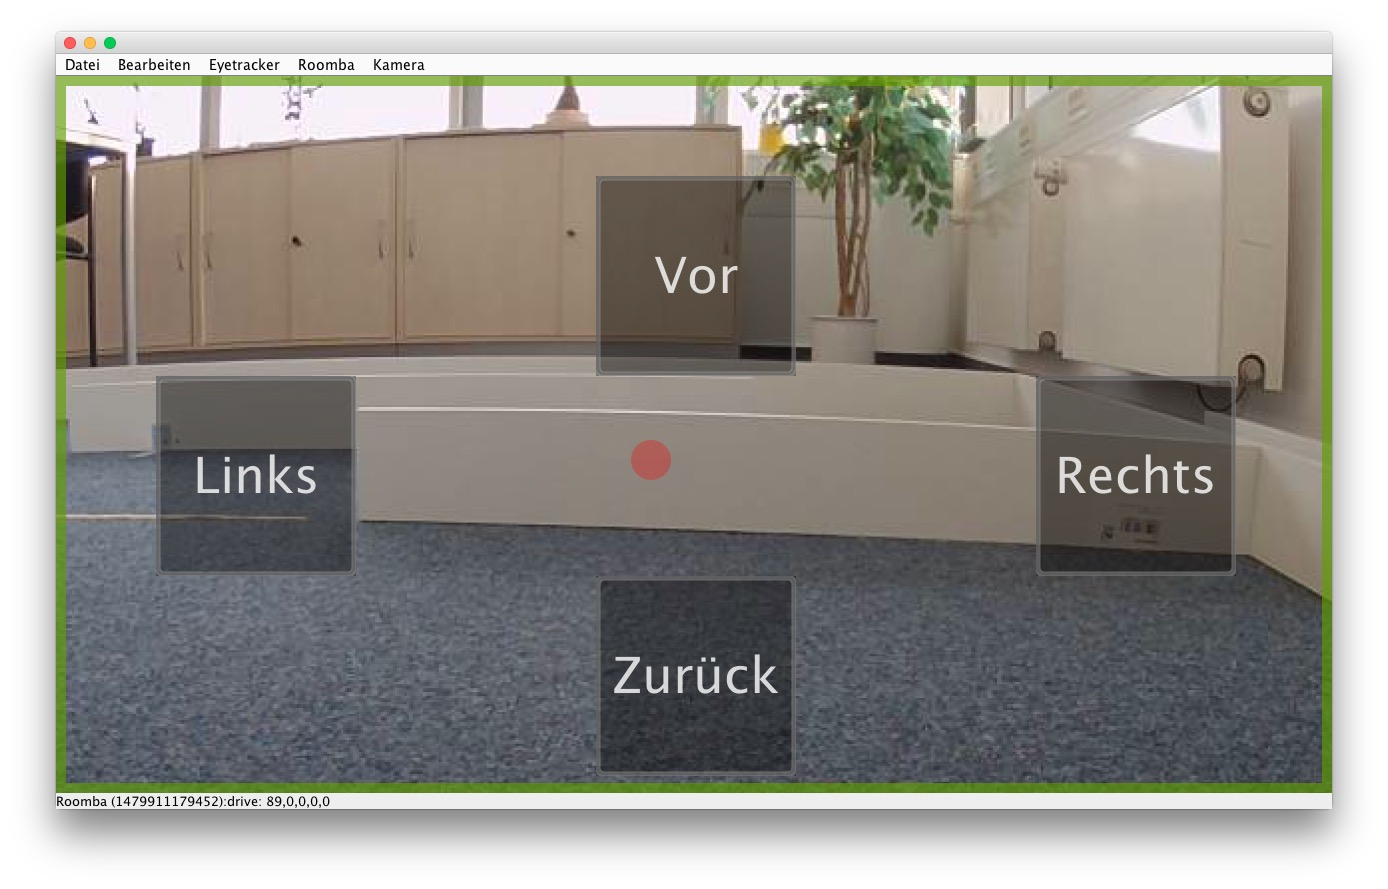
\includegraphics[width=\textwidth, height=100mm]{bilder/implementierung/diskretMode.JPG}
\end{center}
\caption{\textbf{Darstellung der diskreten Steuerelemente} (1) Vor (2) Zurück (3)  Links (4) Rechts. }
\label{fig:diskretMode}
\end{figure}

\subsection{Umsetzung der kontinuierlichen Steuermethode}
\label{subsection:kontSt}
Zur Umsetzung der kontinuierlichen Steuerung wurde ein Art \enquote{Koordinatenkreuz} im Zentrum des Blickbereiches des Benutzers positioniert, siehe Abbildung \ref{fig:contMode}. Hierdurch kann der Benutzer die kontinuierlichen Steuersignale senden und anhand der Ausrichtung des Koordinatenkreuzes die Richtung der Bewegung des mobilen Roboters festlegen. Ein dunkler Bereich in der Mitte des Blickfeldes ist als Stoppbereich konzipiert. Wird der Blick in diesen Bereich gerichtet, bleibt der mobile Roboter unbewegt an seiner aktuellen Position stehen. 
\textcolor{red}{ Algorithmus folgt}
\begin{figure}[ht]
\begin{center}
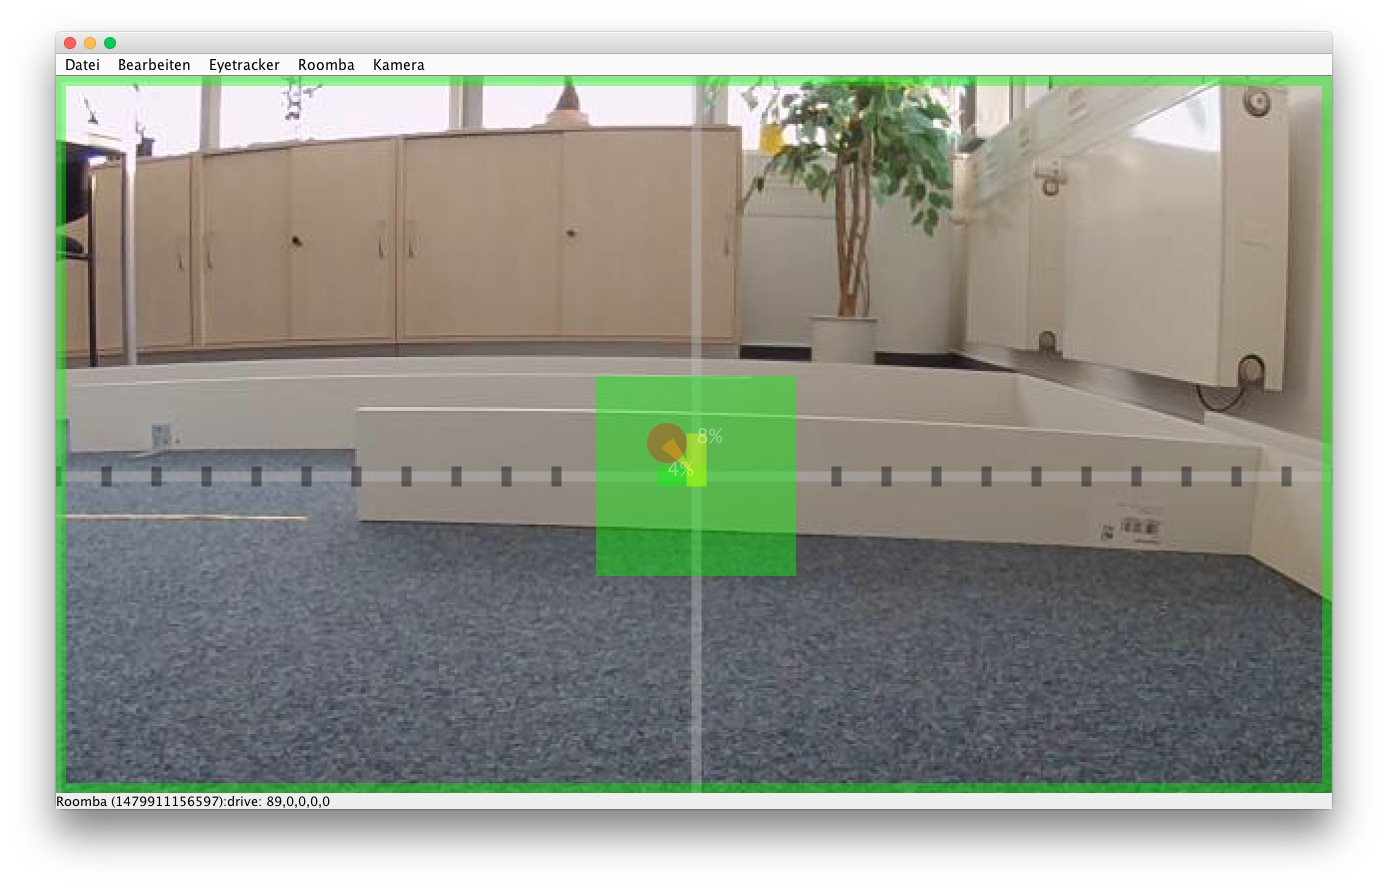
\includegraphics[width=\textwidth]{bilder/implementierung/continuousMode.JPG}
\end{center}
\caption{\textbf{Darstellung der kontinuierlichen Steuerelemente} Zentral ist die Darstellung des Bereiches ohne Steuerbefehle markiert. Man erkennt den ROI durch einen Roten Punkt sowie das }
\label{fig:contMode}
\end{figure}

\section{Eyetracking-System RED von SensoMotoric Instruments GmbH.}
\textcolor{red}{ abschnitt steht noch aus}


\section{Umsetzung der Augengestenerkennung}
\label{section:augengestenerkennung}
\textcolor{red}{
Die Erkennung der Augengesten basiert auf den von Eidam et al. \vgl \cite{Eidam2016} entwickelten Algorithmen und wurde im Rahmen dieser Arbeit übernommen. }
\textcolor{red}{
Es werden fünf Augengesten durch das System erkannt. Hierbei wird die \textbf{horizontale-} und \textbf{vertikale Augengeste} erkennt. Ferner werden der \textbf{Lidschluss} und die \textbf{Fixation} erkannt. Die Erweiterung um eine Blickgeste dient zur Auswahl der Steuerelemente während der Steuerung des mobilen Roboters. Nachfolgend werden die Algorithmen dieser Augengesten dargestellt.}

\subsubsection{Fixation}
\lstset{language=java, numbers=left, caption={Fixation}}
\begin{lstlisting}
int result = Math.abs(maxX - minX) + Math.abs(maxY - minY);  
if (result < maxDispersion && this.size() == maxBufferSize)
return Eyegesture.Fixation;
\end{lstlisting}

\subsubsection{Blickgeste}

\subsubsection{horizontale/vertikale Augengeste}
\lstset{language=java, numbers=left, caption={Algorithmus zur Detektion von horizontalen und vertikalen Augengesten}}
\begin{lstlisting}
//Horizontale Augengestenerkennung  
if (maxDistanceY < maxDisplacement 
	&& maxDistanceX > (monitorWidth - maxDisplacement)) 
	return Eyegesture.HorizontalMove;
    
//Vertikale Augengestenerkennung 
if(maxDistanceX < maxDisplacement 
	&& maxDistanceY > height -maxDisplacement) 
	return Eyegesture.VerticallMove;
\end{lstlisting}

\subsubsection{Lidschluss}
\lstset{language=java, numbers=left, caption={Algorithmus zur Detektion eines Lidschlusses}}
\begin{lstlisting}
if ((zeroCounter > blinkBufferMin) 
	&& ( zeroCounter < blinkBufferMax)) { 
	zeroCounter = 0; 
} 
	return Eyegesture.Blink;
\end{lstlisting}
% * <dokcarlos@icloud.com> 2017-01-22T11:36:54.307Z:
%
% ^.


\section{Umsetzung der Visualisierung eines Motion JPEG Streams}
Die Visualisierung eines Motion JPEG Streams mittels Java wurde durch eine externe Bibliothek implementiert. Hierbei wurde JavaCV verwendet. \textcolor{red}{Details stehen noch aus}

\section{Gestaltung der Benutzeroberfläche}
\textcolor{red}{steht noch aus}

\section{Softwarearchitektur}
\label{section:architektur}

\textcolor{red}{steht noch aus}
\section{Technische Umsetzung}
\textcolor{red}{steht noch aus}
\begin{comment}
\begin{itemize}
  \item Basis:
  \item IDE: Eclipse Mars.2
  \item Software Zielformat
  \item Panikschalter
\end{itemize}


• Java als Programmiersprache • JDK 1.8.0 Update 31 • Swing
\end{comment}


%%%%%%%%%%%%%%%%%%%%%%%%%%%#################################################
%%%%%%%%%%%%%%%%%%%%%%%%%%%#################################################
%%%%%%%%%%%%%%%%%%%%%%%%%%%#################################################
% kapitel5.tex
\chapter{Evaluation}
\label{chapter:evaluation}

\section{Versuchsaufbau}
\label{section:versuchsaufbau}
Im Folgenden werden der Versuchsaufbau, die Versuchsdurchführung und der Evaluationsbogen beschrieben.

\subsection{Komponenten}
Die Komponenten der Steuerung werden in Abbildung \ref{fig:komponenten} (Abbildung Eidam) gezeigt. Der stimuluspräsentierende Bildschirm ist über einen eigenen PC mit der Workstation verbunden. Die Workstation ist mit der ETM konnektiert. Die Workstation führt die iView X Software aus. 

\begin{figure}[ht]
\begin{center}
\includegraphics[scale=0.5]{bilder/evaluation/Aufbau.png}\hfill
\includegraphics[scale=0.4]{bilder/evaluation/Beispiel.png}
\end{center}
\caption{\textbf{Komponenten der Versuchsanordnung} mit einer Ansicht von oben und einer schematischen Darstellung der gleichen Ansicht}
\label{fig:komponenten}
\end{figure}

Bei der Versuchsdurchführung ist auf eine adäquate Sitzpositionierung der Testperson im Verhältnis zum Bildschirm zu achten. Die Augen der Testperson sollten von einer tiefer angeordneten Position der RED observiert werden. Hierbei ist auf ein freies Sichtfeld zu achten. Die schematische Darstellung des Herstellers verdeutlicht die empfohlene Anordnung, siehe Abbildung \ref{fig:empfehlung}. Bei der Durchführung des der Empfehlung des Hersteller werden eine etwa 60 - 80 cm Entfernung

\begin{figure}[ht]
\begin{center}
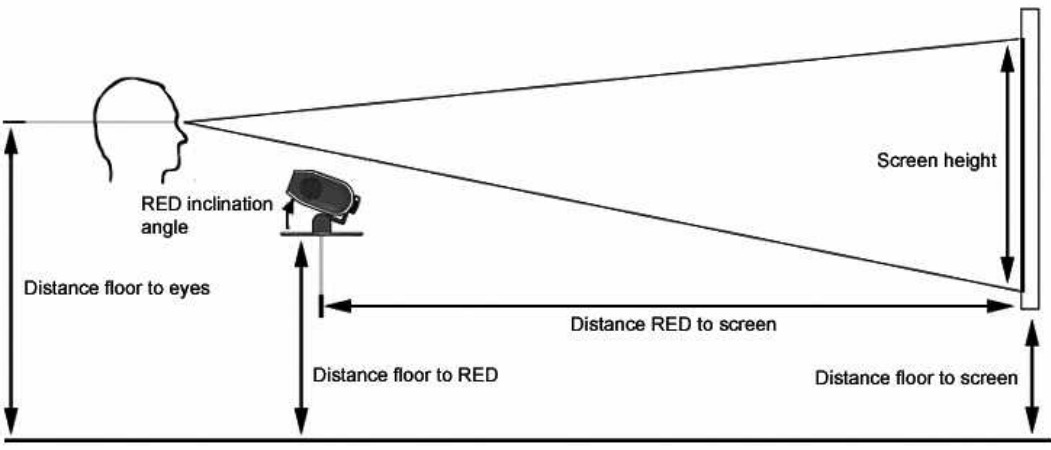
\includegraphics[scale=0.4]{bilder/evaluation/Schema.JPG}
\end{center}
\caption{\textbf{Schema der Empfohlenen Anordnung der Testperson im Verhältnis zur } mit einer Ansicht von oben und einer schematischen Darstellung der gleichen Ansicht }
\label{fig:empfehlung}
\end{figure}

\subsection{Testpersonen}
Für die Durchführung der Parcouraufgabe und der Evaluation des Fragebogens stellten sich vier Personen aus dem Lehrgebiet der Mensch-Computer-Interaktion des Fachbereichs der Mathematik und Informatik der FernUniversität Hagen freiwillig zur Verfügung. Ferner nahm der Verfasser dieser Arbeit ebenfalls an der Evaluation und Parcouraufgabe teil. Die Personen unterschieden sich in ihren Vorerfahrung im Bezug auf die Nutzung von Eyetrackingsystemen. Die Vorerfahrung der Benutzer wurde jedoch nicht weiter differenziert und unterschieden. Jede Testperson bekam vor der Kalibrierung des Eyetrackingsystems eine kurze Einführung in die grundlegenden Funktionsweise der beiden unterschiedlichen Steuerungsmodi und war im Anschluss angehalten nach eigenem Ermessen die Parcourbewältigungsaufgabe durchzuführen.

\subsection{Testparcour}
Der eigentliche Testparcour befindet sich innerhalb eines Bereichs der Größe 200 cm x 200 cm. Hierbei wird der Bereich durch einen 80 cm x 80 cm großen Ladestationsbereich erweitert, Der Zugang zum eigentlichen Parcour ist durch eine Eingangsbarriere der Größe von 40 cm festgelegt. Innerhalb diese Abschnittes ist eine Art \enquote{Kreisbahn} durch eine 50 cm breite \enquote{Strecke} eingerichtet siehe Abbildung \ref{fig:aufbau}

\begin{comment}
\begin{figure}[ht]
    \centering
    \begin{subfigure}[t]{0.52\textwidth}

      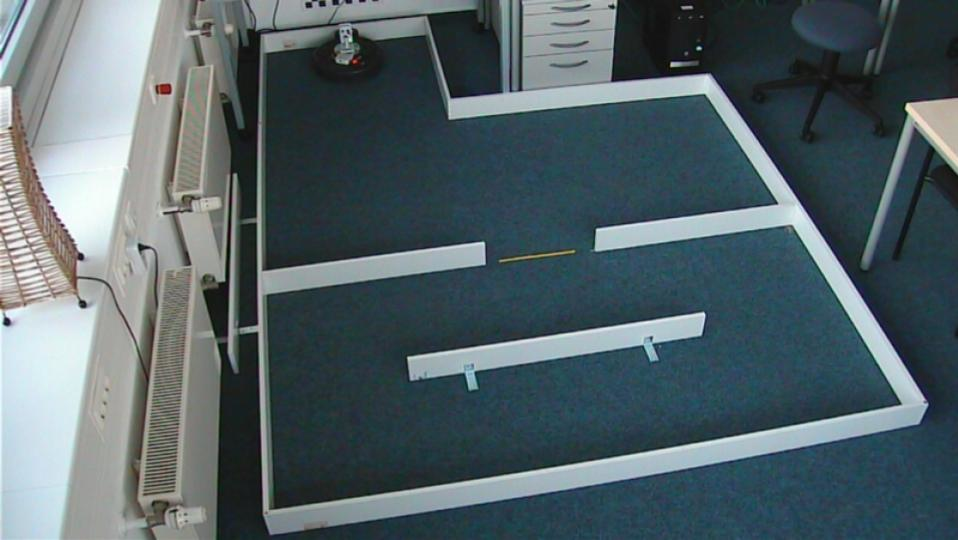
\includegraphics[scale=0.25]{bilder/evaluation/TopView.jpg}
        \caption{Sicht des aufgebauten Parcour}
        \label{fig:parcour}
     
    \end{subfigure}
    \vspace{0.2 cm}
    \begin{subfigure}[t]{0.45\textwidth}
      \includegraphics[scale=0.2]{bilder/evaluation/Parcour.png}
        \caption{zeigt das Auge von hinten mit dem austretendem Sehnerv}
        \label{fig:augeHinten}
    \end{subfigure}
    \caption{Die Muskulatur des rechten Augens}\label{fig:aufbauSchema}
\end{figure}
\end{comment}

\begin{figure}[ht]
\begin{center}
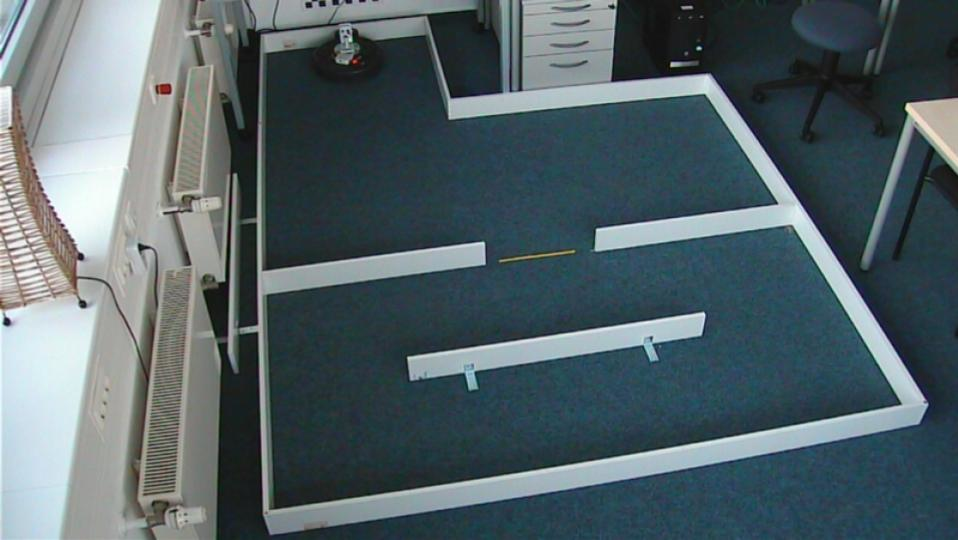
\includegraphics[scale=0.28]{bilder/evaluation/TopView.png}\hfill
\includegraphics[scale=0.2]{bilder/evaluation/Parcour.png}
\end{center}
\caption{\textbf{Parcour Versuchsaufbau} mit einer Ansicht von oben und einer schematischen Darstellung der gleichen Ansicht }
\label{fig:aufbau}
\end{figure}


\section{Versuchsdurchführung}
\label{section:versuchsdurchführung}
Die folgenden Systemeinstellungen wurden von allen beteiligten Testpersonen verwendetet. Die Einstellungen waren für alle beide Steuermethoden verwendet worden. Prinzipiell konnten die Einstellungen frei gewählt werden. Die Benutzer verwendeten alle jedoch die Standardeinstellung:

 \begin{itemize}[Standarteinstellungen]
 \item[-] 1000 ms Fixierungsdauer,
 \item[-] 250 ms minimale Lidschlussdauer und 500 ms maximale Lidschlussdauer,
 \item[-] 200 px maximale Dispersion,
 \item[-] 200 px maximale Auslenkung im Bezug auf die horizontale und vertikale Augengestenerkennung.
 \end{itemize}
 

Zur Messung der Steuerung wurde ein Parcour konzipiert, wobei die zurückgelegte Zeit als quantitatives Messkriterium herangezogen wurde. Ziel dieser Anordnung war es die Aufgabe in einer möglich kurzen Zeit zu bewältigen. Die Vermeidung von Kollisionen war beabsichtigt, jedoch kein Abbruchkriterium bei der Durchführung der Aufgabe. Die Aufgabe galt als erfolgreich beendet, wenn der Parcour ausgehend von der Startmarkierung einmal umfahren und anschließend die Markierung überquert wurde. Die Richtung der Durchführung blieb den Testpersonen überlassen und wurde nicht unterschieden.

Nach Abschluss der Parcouraufgabe wurde zur Klärung der Usability des Prototypen ein Fragebogen mit insgesamt 17 Fragen beantwortet. 



%%%%%%%%%%%%%%%%%%%%%%%%%%%#################################################
%%%%%%%%%%%%%%%%%%%%%%%%%%%#################################################
%%%%%%%%%%%%%%%%%%%%%%%%%%%#################################################








%%%#######################################
%%%#######################################
%%%#######################################
% kapitel2.tex
\chapter{Grundlagen}
\label{chapter:grundlagen}

Traditionelle werden Befehle oder Anweisungen, und damit die eigentliche Kommunikation, vom Mensch zu Computer mittels Computermaus, Tastatur oder Joystick vermittelt. Für Menschen mit körperlichen Einschränkungen speziell bei motorischen Beeinträchtigungen können diese Methoden im Bezug auf die Nutzung Probleme bereiten. Zusätzliche Methoden sind notwendig um dieses Problem zu lösen und damit diesen Menschen einen Zugang zu technischen Anwendungen zu ermöglichen. In den letzten Jahren konnte beispielsweise die Spracherkennung als neue Methode immer besser integriert werden und so Menschen mit Sehstörungen einen effizienteren Zugang ermöglichen. Ein prominentes Beispiel stellt die Firma Apple mit ihrer Spracherkennung namens SIRI zur Verfügung, die auf eine verbale Kommunikation wie von Menschen gewohnt ausgerichtet ist. Aber nicht nur die Sprache und die o.g. Geräte ermöglichen die Kommunikation mit dem Computer. Bei schwer beeinträchtigten Personen mit Bewegungseinschränkungen bleiben oftmals nur die Augen als einziger Kommunikationskanal erhalten um damit mit der Außenwelt oder einem Computersystem zu kommunizieren. Hier haben sich Eytrackingsysteme als hilfreiches Unterstützungssystem bereits in der Praxis bewähren können. Nun ist eine Erweiterung der Kommunikationswege um die Augensteuerung ein wichtiger Schritt jedoch bleibt die Kommunikation häufig auf Monitorsystemen präsentierenden Tastaturtafeln oder Symbolfelder begrenzt und ist häufig abhängig von menschlicher Unterstützung. Damit diese Abhängigkeit die zwangsläufig durch die schwere der Erkrankung gegeben ist reduziert werden kann und um den Grad der Selbstbestimmung und damit auch der Lebensqualität erhöhen zu können, können Robotersysteme die als eine Art Erweiterung der eigenen körperlichen Einschränkungen fungieren und verwendet werden. Die vorliegende Arbeit möchte einen Beitrag leisten um eine Augmentation der körperlichen Möglichkeiten von motorisch beeinträchtigten Personen im Alltag mittels eines Prototypen, der durch die Steuerung eines mobilen Robotersystems die eigene Umgebung erkunden kann. Lebensbereiche erweitert zu ermöglichen.  Einschränkungen durch ein virtuelles    Eine Erweiterung auc. als interessante neue Methode der Kommunikation fungieren. 

Das nachfolgende Kapitel stellt die möglichen Anwendungsgebiete von Eyetracking Systemen und VPS vor. Hierbei stehen Patienten mit Bewegungseinschränkung als Nutzer im Fokus.
%\section{Überblick}
%\label{section:überblick}

\section{Visuelle Mensch-Computer-Interaktion}
\label{section:informationstransfer}

Der Mensch ist ein soziales Lebewesen und auf die Interaktion mit der Umgebung maßgeblich angewiesen. Wird die Möglichkeit der Kommunikation plötzliche genommen stellt dies einen tiefen Einschnitt für das Leben des Betroffenen dar. 

Die vorliegende Abschlussarbeit konzentriert sich auf die Machbarkeit und Nützlichkeit der implementierten Robotersteuerung. Jedoch gelten für die Gestaltung der Benutzeroberfläche grundsätzliche Regeln. Hierbei werden die acht goldenen Regeln Für die Benutzung freundliche Gestaltung interaktiver Schnittstellen von Ben Schneidermann aufgeführt. Ferner werden Norman\'s sieben Grundsätzen beschrieben.






\subsection{Anatomie des Auges}
\subsection{Okulomotorik des Auges}


Die Fovea (Ort des schärfsten Sehens) wird durch schnelle Augenbewegungen ständig auf den beabsichtigen Fixationspunkt im Blickfeld justiert. Die Augenbewegungen werden durch insgesamt sechs Muskeln \ref{} koordiniert und angesteuert. Dabei ist durch die neuromuskuläre Innervation eine hochfrequente und präzise Ansteuerung möglich. Hierbei können verschiedene Klassen von Augenbewegungen unterschieden werden \cite{Joos2003}.  
Joos et. al unterscheidet hierbei (1) Sakkaden, (2) Zielfolgebewegungen und (3) Mikrobewegungen unterschieden. 
Ferner gilt es eine Unterscheidung zwischen Augenbewegung und Blickbewegung zu treffen, da die Aufzeichung der reinen Augenbewegung noch keine Interpreation der Benutzerabsicht ermöglicht. Es muss vielmehr die von der Benutzerin aufgenommene Information bewertet werden,  Der folgende Abschnitt orientiert sich an den Ausführungen von Joos et al. 

%\begin{figure}[ht]
%\begin{center}
%\includegraphics[width=0.49\textwidth, height=55mm]{bilder/grundlagen/auge_vorn.JPG}
%\includegraphics[width=0.49\textwidth, height=55mm]{bilder/grundlagen/auge_hinten.JPG}
%\vspace{-3mm}
%\end{center}
%\caption{\textbf{Die Muskulatur des rechten Augens} (a) als Vorderansicht und (b) zeigt das Auge von hinten mit dem austretendem Sehnerv}
%\label{fig:augenmuskeln}
%\end{figure}

\begin{figure}[ht]
    \centering
    \begin{subfigure}[t]{0.49\textwidth}
        \includegraphics[width=\textwidth, height=60mm]{bilder/grundlagen/auge_vorn.JPG}
        \caption{als Vorderansicht}
        \label{fig:augeVorne}
    \end{subfigure}
    \begin{subfigure}[t]{0.49\textwidth}
        \includegraphics[width=\textwidth, height=60mm]{bilder/grundlagen/auge_hinten.JPG}
        \caption{zeigt das Auge von hinten mit dem austretendem Sehnerv}
        \label{fig:augeHinten}
    \end{subfigure}
    \caption{Die Muskulatur des rechten Augens}\label{fig:rechtesAuge}
\end{figure}

\section{Eyetracker}
\label{section:eyetracker}
Das folgende Kapitel liefert einen Überblick über die Eyetrackingmethoden und die Augen basierte Mensch-Computer Interaktion. Diese Kapitel orientiert sich inhaltlich an den Ausführungen von \cite{Majaranta2014} aus dem Jahre 2014.

Die Augen erfüllen eine zentrale Funktion in der menschlichen Kommunikation. Der Blickkontakt ist oftmals ganz entscheidend für das gegenseitiges Vertrauen. Blickrichtung und Bewegung liefern Einblicke in innere Einstellungen und Absichten von Personen. So sind die Augen, wie man sagt, der Spiegel zur Seele eines Menschen. 

Für Menschen mit Bewegungseinschränkungen sind die Augen oftmals die einzige Kommunikationsmöglichkeit und aus diesem Grund umso entscheidender an der Kommunikation mit der Umgebung beteiligt. Es gibt vielfältige Möglichkeiten wie es zu einer Bewegungseinschränkung mit körperlichen Beeinträchtigungen kommen kann, so können Traumata, Infektiöse Erkrankungen, Erbkrankheiten, Durchblutungsstörungen oder Autoimmunerkrankungen zu einer schwerwiegenden Beeinträchtigung führen. All diese Personengruppen können von unterstützenden technischen Systemen profitieren. Im folgenden wird eine Überblick über die verscheiden Trackingmethoden und Systeme geliefert.


Eyetrackingsysteme sind bereits seit mehreren Jahrzehnten in der Forschung als hilfreiches Werkzeug zur Erforsuchng kognitiver Prozesse und Intentionen der Benutzer in Anwendung. Sie haben Einblicke und Erkenntnisse geliefert welche heute beispielsweise in Marketingbereichen Anwendung finden. Die Benutzung von Eyetrackingssystemen als Eingabemedium scheint eine weitere wichtige Möglichkeit der Nutzung zu sein. Speziell für Menschen mit körperlichen Einschränkungen bieten sich neue Möglichkeiten. So gibt es Blickbasierte- Text Eingabesysteme für Menschen mit Bewegungseinschränkung. Diese Systeme ermöglichen es mittels eines zusätzlichen Kommunikationskanal die Lebensqualität der Benutzer deutlich zu verbessern und ihr Leben ein Stück aktiver zu gestallten.


\subsection{Eyetrackingmethoden}

In den letzten Jahrzehnten wurden die Methoden zur Aufzeichnung von Augenbewegungen kontinuierlich verbessert und weiter entwickelt. Erste Versuche gehen auf Emile Java einen französischen Augenarzt zurück, der sich 1879 mit der Bewegung der Augen beim Lesen beschäftigte. Hierbei benutzte er einen einfachen Spiegel und erkannte durch Selbstversuche, dass verschiedene Phasen während der Augenbewegung zu unterscheiden sind. 
%(https://www.mendeley.com/viewer/?fileId=6a7cfdfc-2054-efc7-174b-68cb892bab31&documentId=2dec1953-63d4-3b07-8bba-0d0beae69ed9). 

Der folgende Abschnitt soll einen Überblick über die häufigsten genutzten Methoden von Eyetracking Systemen liefern. Nach Marajanta et al. \cite{Majaranta2014} spielen hauptsächlich drei Methoden eine Rolle. Dies sind die (1) Videookulographie (VOG), (2) Videobasierten Verfahren und (3) Elektrookulographie. 


\subsubsection{Videookulographie (VOG)}


\subsubsection{Elektrookulographie}
Das Verfahren mittels Elektrookulogram macht sich das Elektrische Potential der Augen repektive der Augenmuskulatur zu nutze. Hierbei werden Elektronen in der Nähe des Auges an der Haut angebracht. Bei der Augenbewegung erzeugte Amplitudendifferenzen konnten zur Detektion von Augenbewegungen herangezogen werden. Der Nachteil dieser Technik liegt in den Kosten der Gerätschaften vor allem des Signalverstärkers sowie an der Tatsache der Positionierung von Elektroden im Gesicht.

\subsubsection{Videobasierten Verfahren}
Eine Weitereentwicklung stellten die videobasierten Systeme dar. Hierbei wird die Augenbewegungen von einer Videokamera aufgezeichnet und zur Erkennung der Augenpositionen verwendet. Hierbei kann sich die Positionierung der Kamera vor dem Betrachter unterscheiden. Es lassen sich am Kopf befestigte Kameras und entfernte Kameras unterscheiden, siehe Figur. 

Der Fokus dieser Arbeit, liegt hierbei auf den Videobasierten Tracking-Systemen.


Unterscheidung zwischen Mobilen und stationären Eyetrackern.
Typischer Aufbau - Kamera nimmt die Bewegungen des Auges auf- Verarbeitender Computer analysiert die Daten und berechnet den POR des Benutzers.

Bei mobilen Eyetrackern befindet sich die Kamera typischerweise unter dem Monitor, bei Mobilen auch head-mountend Systemen genannt ist die Kamera an einem Brillengestell oder einer Helmvorichtung angebracht.
Wichtig \bzgl der Genauigkeit sind die Bildrate und die Auflösung der Videokamera.
Bei Mobilen Systemen befindet sich die Kamera näher am Auge und liefert ein Bild mit mehr Pixels, welches sicher analysiert werden kann.

Faktoren welche die Qualität des Trackings reduzieren sind schlechte Lichtverhöltnisse, Brillengläser, Augenlieder oder Makeup.


\subsection{Anwendungsbereiche von Eyetrackingsystemen}
\label{section:XXX}
\subsection{Anwendungsgebiete in der Medizin}
\label{section:XXX}


\section{Telepräsenzrobotersysteme}
\label{section:XXX}

Für Marvin Minsky war die Entwicklung von Telepräsenzrobotersystemen eine beträchtliche Innovationsmöglichkeit von welcher er bereits in den achtziger Jahren überzeugt war. Zitat Marvin Minsky

Menschen mit Sprach oder Bewegungseinschränkungen benötigen unterstützende Systeme, welche die Lebensqualität durch die Interaktionsfähigkeit verbessern können.

Telepräsenzrobotersysteme sind dadurch charakterisiert, dass die Steuerung durch einen entfernten Benutzer erfolgen kann. Durch die Telepräsenztechnolgie kann der Benutzer die Umgebung des mobilen Roboters mittels einer oder mehrerer angebrachter On-board Kameras virtuell mitverfolgen. Eine Software am eigenen Computer ermöglicht die Steuerung des Roboters aus der Ferne. Der Benutzer fühlt sich aufgrund dieser Möglichkeiten an diesem Ort des Roboters präsent, obwohl sich der Benutzer an einem weit anderen Ort aufhalten kann. (Sheridan TB: Telerobotics, automation and human supervisory control. 1992, Cambridge: The MIT press)

\tp existieren bereits seit den 1990 Jahren. (Literatur???)
Der Fortschritt in der Informations- und Kommunikationstechnik haben die Entwicklung von \tp im Gesundheitswesen ermöglicht. (Fels DI, Weiss PLT: Video-mediated communication in the classroom to support sick children: a case study. Int J Ind Ergon. 2001, 28: 251-263. 10.1016/S0169-8141(01)00020-8.) (Thacker PD: Physician-robot makes the rounds. JAMA: The Journal of the American Medical Association. 2005, 293: 150-150.).

Der Nutzen der Systeme zeigt sich in verschiedenen Anwendungsgebieten. Der folgende Abschnitt orientiert sich stark an den Ausführungen von \cite{Kristoffersson2013}.

\subsection{Anwendungsgebiete im Überblick}
\label{section:XXX}

Die Anwendung von \tp wurde für verschiedene Anwendungsgebite und Szenarien beschrieben. So beschreibt \cite{Kristoffersson2013} Anwendungsgebiete im Bereich der Medizin, aber auch in Umfeld von Bürotätigkeiten. 

Grundsätzlich werden 2 Anwendungsszenarien für den Gebrauch von \tp benutzt. So beschreibt 
\subsection{Anwendungsgebiete in der Medizin}
\label{section:XXX}
\subsection{Steuerungen von Robotersystemen}
\label{section:XXX}

Besteht ein Beispiel für eine Fußnote.\footnote{Eine Anmerkung die nicht in den oben beschriebenen Text passt.}

\subsection{Roomba}
Der Roomba ist ein autonomer Staubsaugerroboter der von der iRobot Corporation hergestellt wird. Der Roomba wurde dafür konzipiert ohne einen Computer und ohne technische Vorkenntnisse des Benutzers zu funktionieren. Seit 2005 gibt es eine offenen Schnittstellendokumentation Womit es möglich wurde den Roboter im Verhalten vollständig zu kontrollieren.

Die ihr Vorwort Cooperatiion, welche den Roomba herstellte erkannte im Dezember 2005, das der Wunsch bezüglich einer Individuellen Steuerung des Roboters gegeben ist und brachte die Dokumentation zur zur Steuerung das Serial Command Interface (SCI) heraus. Später Würde dies im Roomba Open Interface (ROI) umbenannt.

\subsubsection{Roomba Modi}
Bei der Benutzung des ROI befindet sich der Roomba in einer von fünf verschiedenen Modi. Die Zustände legen fest welche Verhaltensweisen das tun was möglich sind und wie auf eintreffende ROI Befehle reagiert wird. Folgend werden die fünf Zustände kurz beschrieben:

Schlafmodus:Der Roomba reagiert Nicht auf eintreffenden Befehle, Kann jedoch mittels power Button aktiviert werden.

An: Roomba ist wach und wartet auf den Startbefehl. in diesem Zustand verhält sich der Rumba normal und Kann mittels Tasten oder Fernsteuerung kontrolliert werden. Mittels Start Befehl kann der Modus geändert werden.

Passiv: Der Roomba hat das Startsignal erhalten. in diesem Modus können die Sensoren ausgelesen werden jedoch ist keine Steuerung Über die Schnittstelle möglich. Die Tasten des Roomba abeiten normal. 

Safe: der Rumba hat das Kontrolle Signal vom Passiven Modus oh Damen das Safe Signal vom Fullmodus erhalten. Alles was im Passiven Modus möglich war ist weiterhin möglich zusätzlich kann der Roomba kontrolliert und gesteuert werden. die Tasten des Wunders können das Verhalten nun nicht mehr ändern jedoch können die Tasten durch die Sensor Daten erfasst werden. Alle möglichen Befehle sind nun ausführbar. Ein Sicherheitsmodus ist bereits vor installiert um zu vermeiden, dass der Roomba Sicht gefährden. Die Sicherheitseinstellungen werden ausgelöst sobald der Roomba einer der folgenden Ereignisse wahrnimmt:
Ein AbhangBeim vorwärts fahren oder Rückwärtsfahren wird erkannt
Ein Rad steckt fest.
Das Ladegerät ist angeschlossen und wird geladen
Falls eine dieser Ereignisse festgestellt wird wird der Roomba zurück in den Passivmodus versetzt. 

Full: Durch einen Full-befehl im Safe Modus Wird dieser Zustand eingenommen. In diesem Modus gibt es die gleichen  Möglichkeiten wie im Safe Modus bis auf die Tatsache, dass die sicherheitsrelevanten Features ausgeschaltet sind. Das Senden des Befehls SPOT, CLEAN oder MAX bringen den Rumba in den Passivmodus. Das Drücken des virtuellen Powerknopf das führt dazu dass der Roomba in den Passiv Modus wechselt und dann in den Schlafmodus wechselt. 
(Nachfolgend einfügen der Darstellungen aus dem Hackers-Buch)

\subsubsection{Roomba Befehlsstruktur}
All ROI commands start with a command opcode, a single byte with a value between 128 (0x80) and 143 (0x8F), inclusive. Only 16 opcodes have been published, but these 16 allow almost complete control. There may be more, unpublished opcodes. In addition to the command opcode byte, an ROI command may include one or more data bytes that are arguments to the command. Many commands, like the START command, consist of only the command opcode byte and no data bytes. The PLAY command is an example of a command that takes one extra command byte, a data byte with the number 1–16 of the song to play. All commands except the SONGcommand have a fixed number of data bytes. The SONG command has a variable number of data bytes, depending on the length of the song, N. The number of data bytes is determined by the formula 2+2N. Therefore, if the song to be sent is one note long (N=1), the number of data bytes to send is 4. For a 10-note song (N=10), 22 data bytes are sent. To send a complete ROI command, send the appropriate command byte and the appropriate data bytes, if any, from the serial port of your controlling computer and to the RXD pin of the
%%%#######################################
%%%#######################################
%%%#######################################
\begin{itemize}
\item \textbf{01.10.16 - Meilenstein 1}: Anmeldung der Bachelorarbeit beim Prüfungsamt. 
Konzept der Arbeit fertigstellen und Unklarheiten besprechen. Titel der Arbeit festlegen.
Evaluationsinhalte festlegen und Falsifikationen dieser besprechen.
Software-Testversion - Stabilität ausreichend zur Evaluation der Basis-Steuerung + Codeoptimierung + Testfälle besprechen. 


\item  \textbf{01.11.16} - 1. Besprechung Stand der Arbeit mit folgenden Themen:
 \textbf{Meilenstein 2:} Software-Version zur Evaluation abschließen.
Fertigstellung des Kapitels Einführung. 
Fertigen Evaluationsbogen besprechen und ggf. anpassen.


\item  \textbf{01.12.16} - 2. Besprechung Stand der Arbeit.
Fertigstellung des Kapitels Grundlagen
Evalutationsergebnises besprechen.

\item  \textbf{02.01.17} - 3. Besprechung Stand der Arbeit.
Fertigstellung Kapitel Implementierung: Besprechung von unklaren Formulierungen, Visualisierungsmöglichkeiten,

\item  \textbf{01.02.17} - 4. Besprechung Stand der Arbeit.
 \textbf{Meilenstein 3:} Fertigstellung der ersten Version der Abschlussarbeit nach Abschluss von Kapitel Evaluation und Zusammenfassung: Besprechung des Literaturverzeichnis

\item  \textbf{02.03.17} - 5. Besprechung Stand der Arbeit.
 \textbf{Meilenstein 4:} Fertigstellung der Endgültigen - Version der Abschlussarbeit nach Korrekturlesung und Anpassung der geschlechtsneutralen Sprache.

\item \textbf{31.03.17 - Meilenstein 5:} Abgabe der Bachelorarbeit beim Prüfungsamt. \begin{itemize}
\item schriftliche Ausarbeitung in Papierform inklusive der im Anhang der Ausarbeitung unterschriebenen Erklärung zur selbstständigen Arbeit.
\item Software.
\item Daten, wie bspw. Ergebnisse von Experimenten oder generierte Bilddaten.
\item die schriftliche Ausarbeitung in elektronischer Form als PDF-Datei samt Quelldateien wie bspw. Bilder oder Diagramme. 
\end{itemize}
\item 01.04.2017 - Präsentationvorbereitung.
\item 07.04.2017 - Präsentationskonzept besprechen. 
\item 21.04.2017 - Fertige Präsentation abgeben.
\item \textbf{XX.XX.2017 - Meilenstein 6} Kollegiumsvortrag halten. 

\end{itemize}


%%%%
%Woche 14 & KW 1 &  \checked & & - \\
%Woche 15 & KW 2 &  \checked & & - \\
%Woche 16 & KW 3 &  \checked & & - \\
%Woche 17 & KW 4 &  \checked & & - \\
%Woche 18 & KW 5 &  \checked &  & - \\
%Woche 19 & KW 6 &  \checked & & - \\
%Woche 21 & KW 7 &  \checked &  & - \\
%Woche 22 & KW 8 &  \checked & & - \\
%Woche 23 & KW 9 &  \checked &  & - \\
%Woche 24 & KW 10 &  \checked && - \\
%Woche 25 & KW 11 &  \checked & & - \\
%Woche 26 & KW 12 &  \checked & & - \\
%Woche 27 & KW 13 &  \checked & & - \\
%Woche 28 & KW 14 &  \checked & Abgabe der Bachelorarbeit einen sehr langen Text der die Seite vermutlich vergrößert beim Prüfungsamt es wird einfach noch länger um zu schauen was passiert. & - \\
%Woche 29 & KW 15 &  \checked & Abgabe der Bachelorarbeit beim Prüfungsamt. & - \\
%Woche 30 & KW 16 &  \checked & Abgabe der Bachelorarbeit beim Prüfungsamt. & - \\
%Woche 29 & KW 15 &  \checked & Abgabe der Bachelorarbeit beim Prüfungsamt. & - \\
% Woche 30 & KW 16 &  \checked & Abgabe der Bachelorarbeit beim Prüfungsamt. & - \\
%Woche 29 & KW 15 &  \checked & Abgabe der Bachelorarbeit beim Prüfungsamt. & - \\
%Woche 30 & KW 16 &  \checked & Abgabe der Bachelorarbeit beim Prüfungsamt. & - \\
%\hline\\
%\multicolumn{5}{c}{Abschlussnote}\\
%\bottomrule

\newenvironment{mycompactitem}{%
  \begin{compactitem}%
  }{%
  \strut\end{compactitem}%
}

\newcolumntype{P}[1]{>{\begin{minipage}[t]{#1}\raggedright\arraybackslash}p{#1}<{\end{minipage}}}
\renewcommand\arraystretch{1.25}

\begin{longtable}{P{3cm}P{3cm}P{6cm}@{}}
\textbf{Gebiet}&  \textbf{Gebiet} & \textbf{Erläuterung} \\
  Gebiet 1 &
    \begin{mycompactitem}
      \item Punkt 1 
        \begin{compactitem}
          \item Unterpunkt 1
          \item Unterpunkt 2
          \item etc.
        \end{compactitem}
      \item Punkt 2
      \item Punkt 3
      \item Punkt 4
    \end{mycompactitem} \\
  Gebiet 2 & 
    \begin{mycompactitem}
      \item Punkt 1 
      \item Punkt 4
    \end{mycompactitem} \\
  Gebiet 3 & 
    Hier steht Text\\
  Gebiet 4 mit weiterer Erläuterung & 
    Hier steht Text 
      \begin{mycompactitem}
        \item Punkt I
        \item Punkt II
      \end{mycompactitem} 
\end{longtable}


 \begin{longtable}{|l|r|c|p{2cm}|}
 \hline
 Linksbündige Spalte.&Rechtsbündige Spalte&Zentrierte Spalte&Parbox\\
 \hline
 Kurzer Text.&Kurzer Text.&Kurzer Text.&Kurzer Text.\\
 \hline
 Text.&Text.&Text.&In diesem Felde nun ein elendslanger Text, um Umbrüche innerhalb eines Feldes zu erzeugen.\\
 \hline
 Text.&Text.&Text.&der Befehl $\backslash$vspace*\{\} weiter oben im Quellcode hat einen Umbruch vor dieser Zeile bewirkt.\\
 \hline
 \end{longtable}
 
 (360$^\circ$)